%!TEX root = ../../../adrien_gomar_phd.tex

\subsection{Presentation}
\label{sub:dream_ls_ael_presentation}

Two structural modes are considered for the aeroelastic study of this 
configuration: the second bending/flexion mode and the first torsion mode
of the front rotor. These were inputs of the current work.
The shape of the modes is shown in Fig.~\ref{fig:dream_ls_ael_modes}
with an arbitrary amplitude, large enough to ease the visualization.
Two inflection lines are seen for the 2F mode, while only
one is seen for the 1T, hence their designation.
\begin{figure}[htp]
  \centering
  \subfigure[2F]{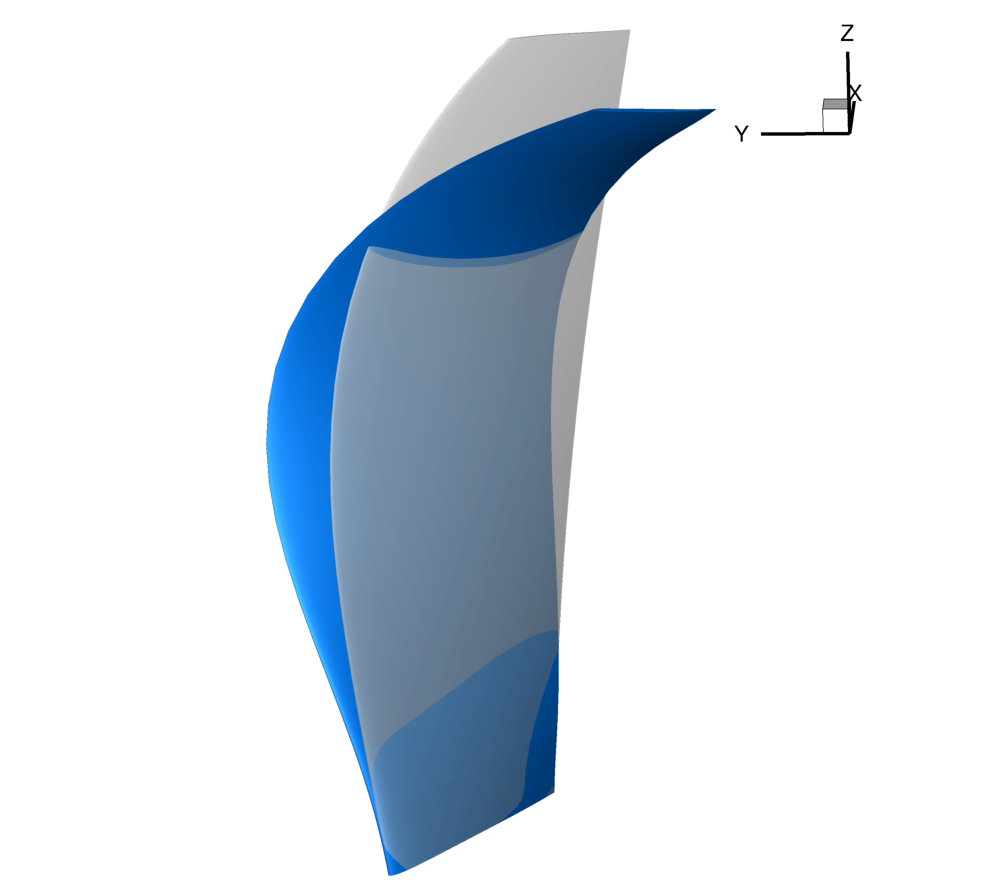
\includegraphics[height=.35\textwidth]{mode_2F.png}}
  \subfigure[1T]{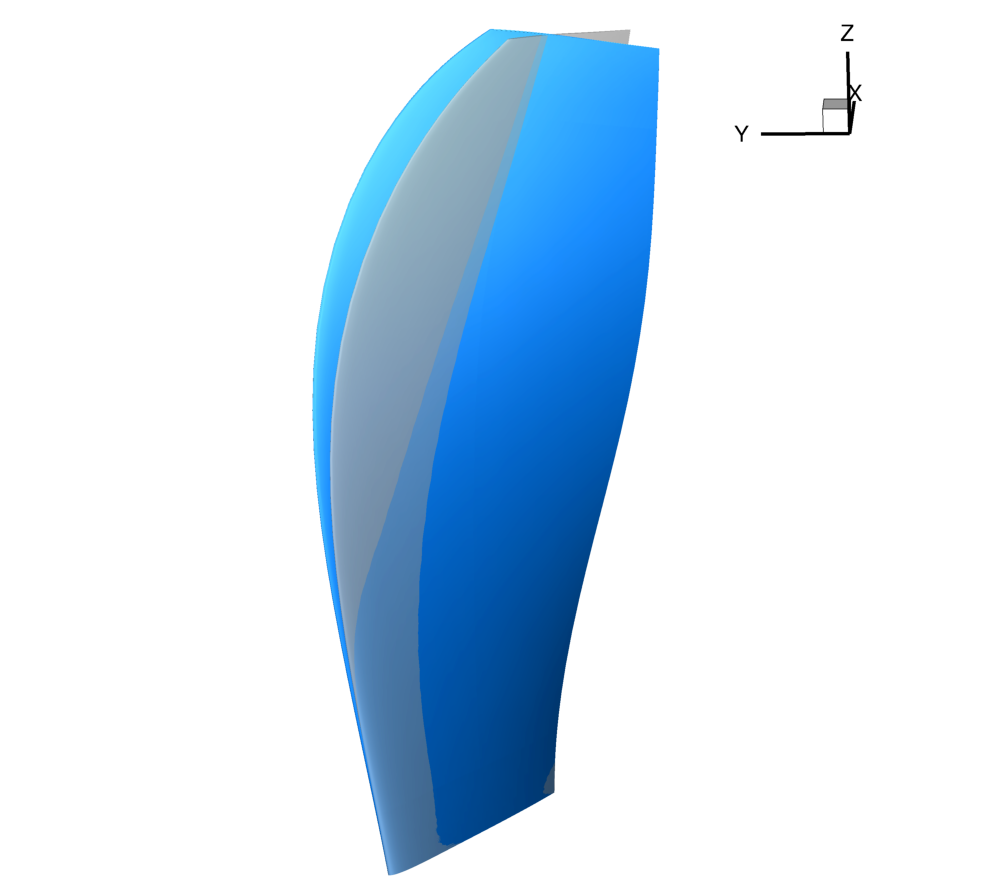
\includegraphics[height=.35\textwidth]{mode_1T.png}}
  \caption{Low-speed isolated configuration: structural modes considered.}
  \label{fig:dream_ls_ael_modes}
\end{figure}
The frequency, mass and stiffness of the modes 
are given with the corresponding modes.
The frequency of each modes varies between 
$495~\textrm{Hz} \leq f_{AEL} \leq 600~\textrm{Hz}$
while the blade passing frequency of the opposite rows,
namely the rear rotor, is $1913~\textrm{Hz}$. However,
this last frequency governs the unsteady rigid flow physics 
and will have to be computed along with the aeroleastic frequency.
Therefore, the multi-frequential formulation of the
harmonic balance approach will be used in the following.

\subsection{Numerical setup}
\label{sub:dream_ls_ael_number}

The \emph{elsA} CFD flow solver is 
used (see Appendix~\ref{app:elsa}) along with its AEL module.
Again, only a one-blade passage domain is used.
Phase-lag boundary conditions are therefore used
and each computed frequency is associated to one phase-lag~\cite{ThesisGuedeney}.
For the aeroelastic modes, 
four nodal diameters are considered, corresponding to IBPA
values of: $[-60^\circ, -30^\circ, 30^\circ, 60^\circ]$. 
The aeroelastic coupling is considered to be linear (weak coupling
approach), therefore a very small amplitude of the mode is applied
and the fluid response is analyzed.

Due to the non-linearity of the Navier--Stokes
equations, combinations of 
the two base frequencies (blade passing frequency and
aeroelastic frequency) can emerge in the front rotor. 
This leads to a set of possible frequencies that 
is two-dimensional. An infinite number of frequencies
can not be computed meaning that this set 
has to be truncated. In the electronic literature,
\citet{Kundert1988} propose two types of truncation:
the "square grid" and the "diamond grid" truncations.
These are schematically represented in Fig.~\ref{fig:dream_hb_truncation}.
Dots represent frequencies that are computed by the multi-frequential
harmonic balance approach.
\begin{figure}[htp]
  \centering
  \subfigure[square grid]{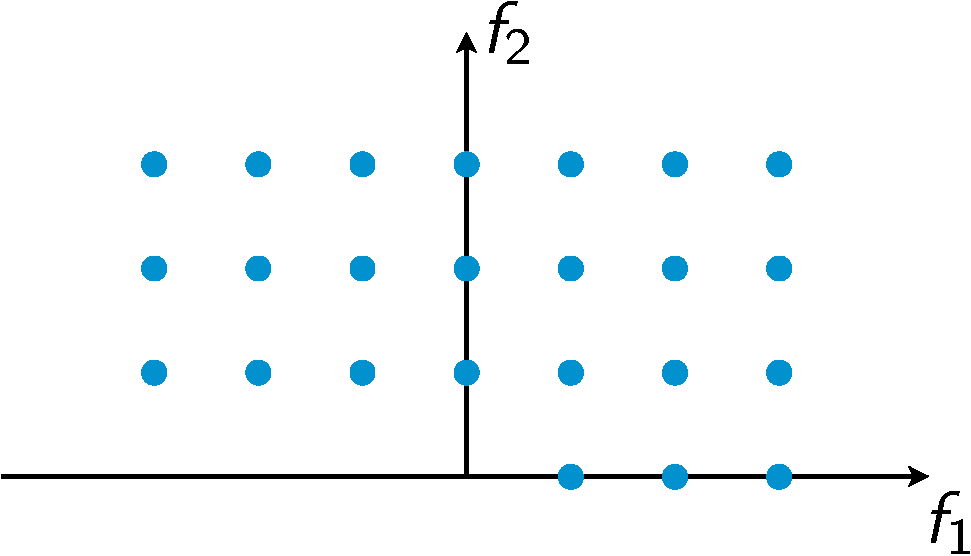
\includegraphics[width=.25\textwidth]{truncation_square.pdf}}
  \subfigure[diamond grid]{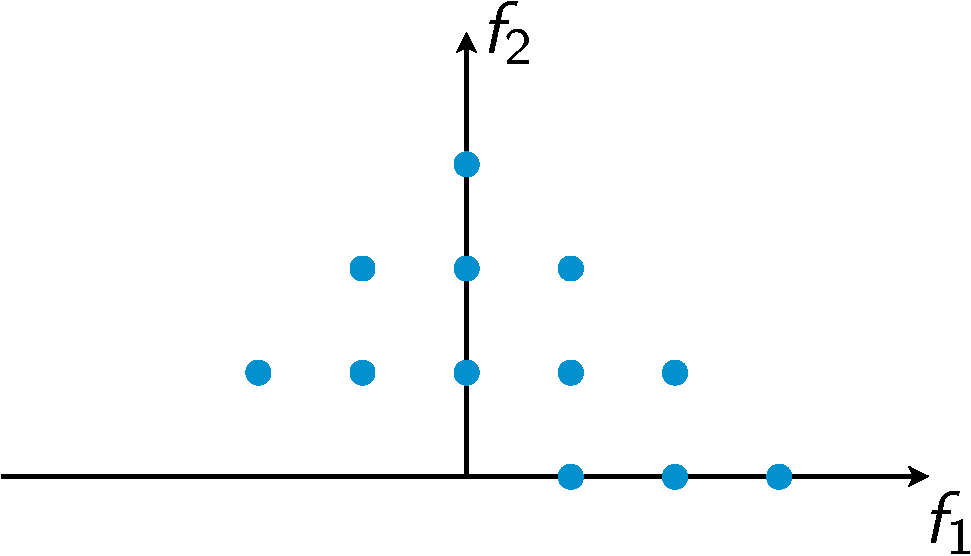
\includegraphics[width=.25\textwidth]{truncation_diamond.pdf}}
  \subfigure[cross grid]{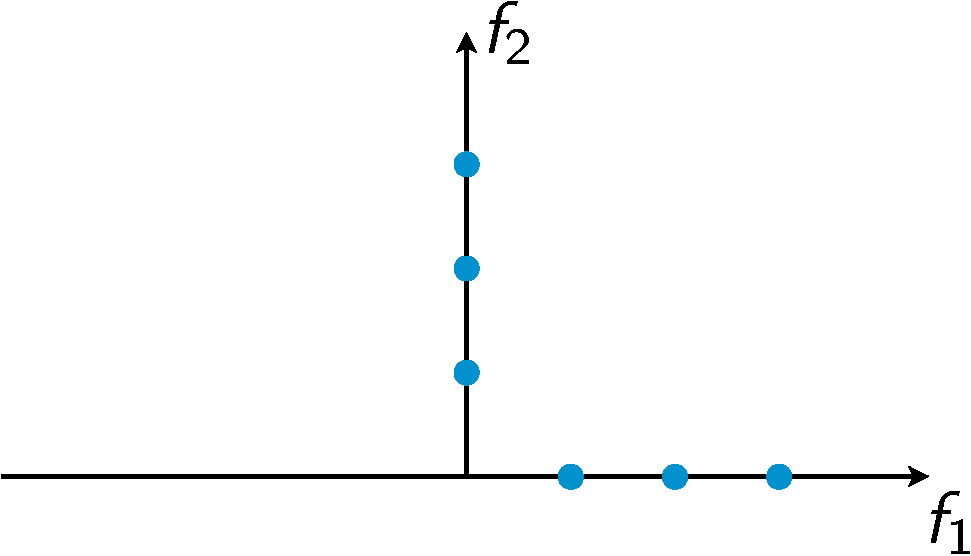
\includegraphics[width=.25\textwidth]{truncation_cross.pdf}}
  \caption{Truncation grids for reducing the set of frequencies of multi-frequential
  harmonic balance computations.}
  \label{fig:dream_hb_truncation}
\end{figure}
In the turbomachinery literature, \citet{Gopinath2007} follows the
diamond grid pattern while \citet{Ekici2007} seems to choose a
square grid pattern. In his PhD thesis, \citet{ThesisGuedeney}
first choose the frequencies by knowing which one emerge based on
a reference classical time-marching computation. Of course,
this approach can only be done \emph{a posteriori} which limits
the predictability of the method. He
also made computations with a "cross grid" truncation 
(shown in Fig.~\ref{fig:dream_hb_truncation}), this new type 
of truncation scheme only considers the harmonics of the
base frequencies. \citet{ThesisGuedeney} showed that this
truncation pattern gives
similar if not better results that the
"diamond grid" truncation pattern. 

In this work, the two frequencies 
have a different physical meaning. In fact, while the blade passing frequency
has been shown to convey the main flow physics (potential effects, wakes, 
tip vortices to name but a few), the aeroelastic frequency is more likely
to influence the near blade wall flow field. In fact, as recalled
previously, the amplitude of vibration is kept very small,
yielding a local influence of the blade vibration.
Therefore, in this work, it seems reasonable to choose a "cross grid"
truncation pattern.

Finally, the harmonic balance computations are run with
five frequencies in total. In the rear rotor,
the harmonics of the front rotor blade passing frequency
are chosen. In the front rotor, the first frequency is the
frequency associated to the vibration of the blade and the
remaining ones are harmonics of the rear rotor blade 
passing frequency.

The time instances are automatically chosen using the OPT
algorithm (see Sec.~\ref{sec:algo_opt}) which leads to 
a condition number always lower than $1.1$ which ensure
the convergence of the computations.

\subsection{Stability curve}
\label{sub:dream_ls_ael_curve}

The stability curve, namely the 

\subsection{Local damping}
\label{sub:dream_ls_ael_local_damping}